\chapter{Wygląd i przepływ w aplikacji}

Interfejs użytkownika zaprojektowano z myślą o natychmiastowej obsłudze przy wykorzystaniu czytelnych kafelków i przycisków interaktywnych. Po uruchomieniu, aplikacja wyświetla centralny widok, z którego możemy skierować się na procedurę dodania nowego pracownika, lub przejść do terminala uwierzytelniającego.

\section{Widok Główny - Menu Nawigacyjne}
Główny ekran to przejrzysty \textit{Dashboard} pozwalający na wybór kierunku działania aplikacji.

\begin{center}
    % TUTAJ WKLEJ ZDJĘCIE MAIN_MENU (Uruchom aplikację, wejdź na ekran początkowy i zrób screena)
    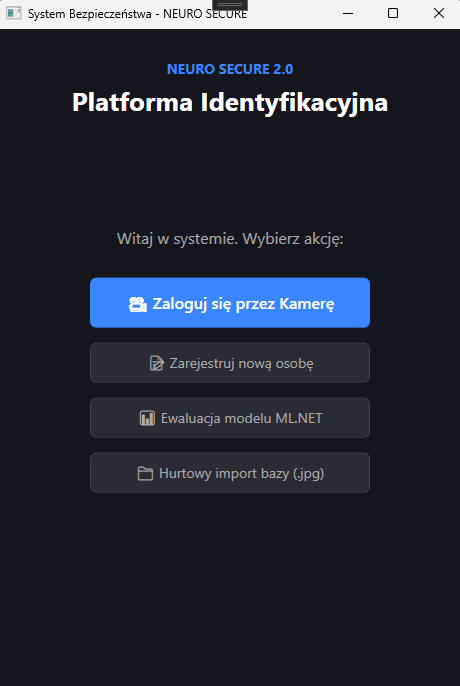
\includegraphics[width=0.55\textwidth]{img/ui/menu_glowne.png}
    \captionof{figure}{Menu powitalne aplikacji FaceAuthApp. Możliwość przejścia do modułu autoryzacji lub do zarządzania bazą danych twarzy.}
\end{center}

\section{Rejestracja Profilu Biometrycznego}
Ekran rejestracji pozwala administratorowi skonfigurować dowolne źródło wizji (z listy podłączonych kamer USB w systemie) bądź ręcznie wprowadzić gotowe, zweryfikowane zdjęcie twarzy bezpośrednio z dysku nośnika. Po przypisaniu etykiety (np. Imię i Nazwisko pracownika) i kliknięciu przycisku zapisania, program błyskawicznie przetworzy zdjęcie przez sieć neuronową i zabezpieczy je w ustrukturyzowanym pliku bazy w postaci nienaruszalnego wektora cech. Dodatkowo, w ukrytym katalogu \texttt{Dane} utworzy się profilowy zrzut na wypadek konieczności ponownego uczenia systemu.

\begin{center}
    % TUTAJ WKLEJ ZDJĘCIE REJESTRACJI 1 (Ekran rejestracji z wpisanym imieniem)
    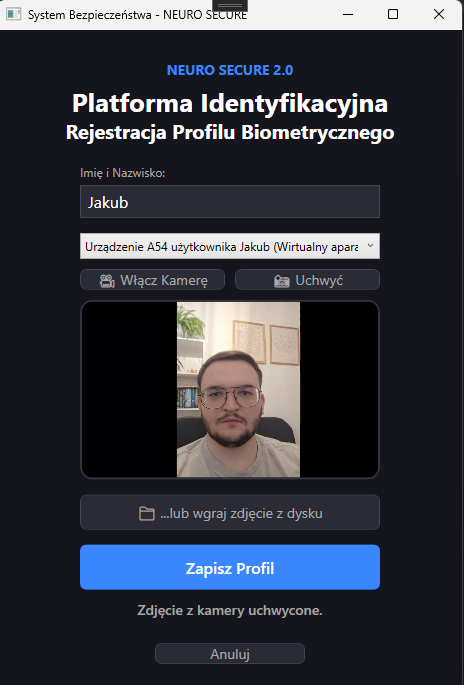
\includegraphics[width=0.55\textwidth]{img/ui/rejestracja_1.png}
    \captionof{figure}{Ekran rejestracji z wpisanym imieniem i wczytanym zdjęciem referencyjnym.}
\end{center}

\begin{center}
    % TUTAJ WKLEJ ZDJĘCIE REJESTRACJI 2 (Potwierdzenie zapisu na zielono)
    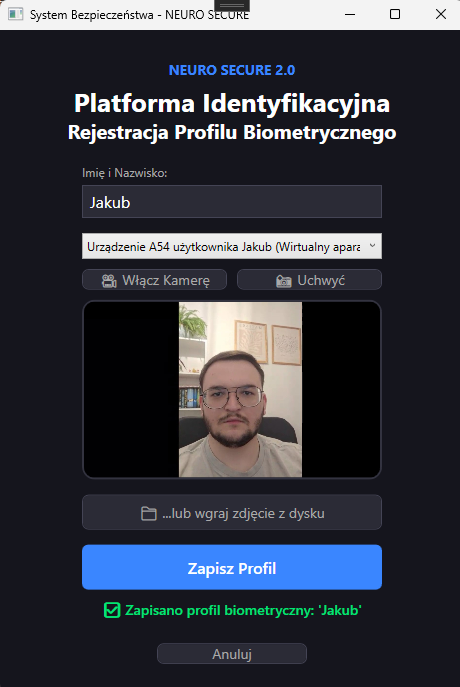
\includegraphics[width=0.55\textwidth]{img/ui/rejestracja_2_success.png}
    \captionof{figure}{Potwierdzenie zapisu profilu pracownika do bazy biometrycznej na podstawie cech twarzy.}
\end{center}

\section{Hurtowy Import Bazy Danych}
W zaawansowanych scenariuszach wdrożeniowych, administratorzy mają możliwość masowego załadowania wcześniej zweryfikowanych pakietów zdjęć. Aplikacja weryfikuje każde zdjęcie z osobna i automatycznie wpina je do rejestru wektorowego.

\begin{center}
    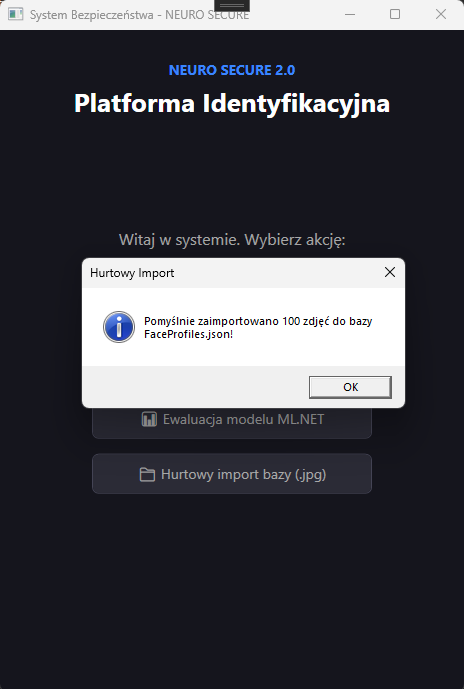
\includegraphics[width=0.55\textwidth]{img/ui/hurtowy_import.png}
    \captionof{figure}{Raport z błyskawicznego, hurtowego importu setek zdjęć autoryzowanych pracowników prosto z dysku twardego.}
\end{center}

\section{Terminal Logowania i Kalibracja Threshold}
Główny moduł autoryzacyjny. Proces autoryzacji został wyposażony w płynny suwak weryfikacji (\textit{Security Level Threshold}). Określa on krytyczną wartość wyrażaną w procentach.
W trybie swobodnym można obniżyć wymóg np. do $65\%$ – system będzie bardziej tolerancyjny na inne oświetlenie czy okulary. Jeśli ochraniamy środowisko wysokiego ryzyka (np. serwerownię), zmiana wartości suwaka do $85\%$ sprawi, że jedynie idealne, frontalne odzwierciedlenie twarzy bez elementów rozpraszających da pozytywny rezultat, rygorystycznie minimalizując ryzyko błędnej akceptacji (False Acceptance Rate).

\begin{center}
    % TUTAJ WKLEJ ZDJĘCIE LOGOWANIA 1 (Ekran skanowania z suwakiem na np 70%)
    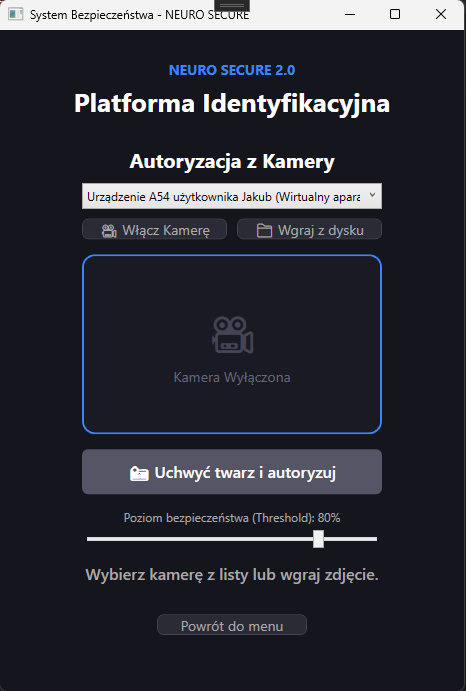
\includegraphics[width=0.55\textwidth]{img/ui/logowanie_ekran_suwak.png}
    \captionof{figure}{Moduł uwierzytelniający z panelem regulacji czułości wariancji algorytmu Cosine Similarity. Na ekranie widać aktywny pogląd lustrzany z obiektywu operatora.}
\end{center}

\begin{center}
    % TUTAJ WKLEJ ZDJĘCIE LOGOWANIA SUCCESS (Kiedy zaloguje kogoś poprawnie)
    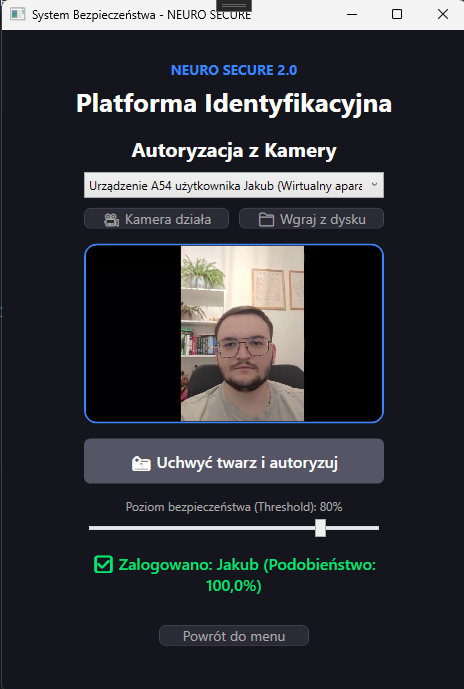
\includegraphics[width=0.55\textwidth]{img/ui/logowanie_granted.png}
    \captionof{figure}{Pomyślne potwierdzenie tożsamości z wyliczonym wskaźnikiem dopasowania (zielony komunikat na dole ekranu).}
\end{center}

\begin{center}
    % TUTAJ WKLEJ ZDJĘCIE LOGOWANIA DENIED (Gdy twarz nie pasuje do wzorca, błąd na czerwono)
    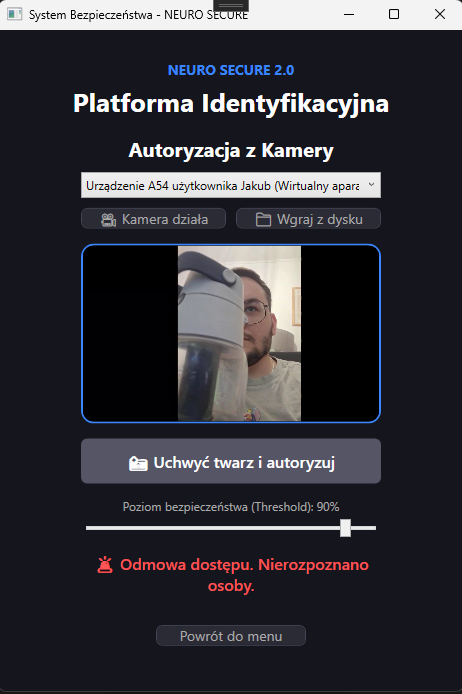
\includegraphics[width=0.55\textwidth]{img/ui/logowanie_denied.png}
    \captionof{figure}{Odrzucenie intruza z powodu niedostatecznego wyniku podobieństwa do jakiegokolwiek wzorca z bazy.}
\end{center}

\begin{center}
    % TUTAJ WKLEJ ZDJĘCIE LOGOWANIA SPOOFING (Przy próbie zasłonięcia kamerki kartką lub przyłożeniu płaskiego telefonu - wykrycie braku wariancji)
    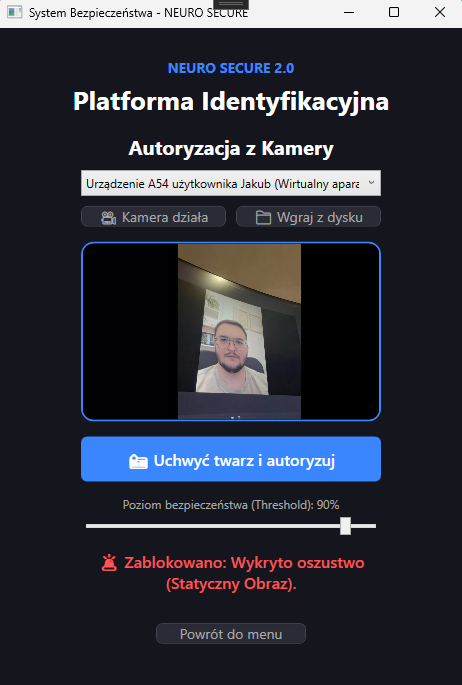
\includegraphics[width=0.55\textwidth]{img/ui/logowanie_spoofing.png}
    \captionof{figure}{Blokada obronna Anti-Spoofing nałożona w momencie wykrycia absolutnie statycznego obiektu przed obiektywem.}
\end{center}
